%\begin{enumerate}[label=\thesection.\arabic*.,ref=\thesection.\theenumi]
%\numberwithin{equation}{enumi}
\item Using Nyquist criterion, find out the range of K for which the closed loop system will be stable.
\begin{align}
\label{eq:ee18btech11016_system}
 G(s)=\frac{K(s+2)(s+4)}{s^2-3s+10} ;  H(s) = \frac{1}{s}  
\end{align}
\\
\solution  The system flow can be described by Fig. \ref{fig:ee18btech11016_figure1}
\begin{figure}[!ht]
    \begin{center}
        \resizebox{\columnwidth}{!}{\input{./figs/ee18btech11016_figure1.tex}}
    \end{center}
    \caption{}  
    \label{fig:ee18btech11016_figure1}
\end{figure}
%\item Find the open loop transfer function G(s)H(s)
%\\
%\solution 
From \eqref{eq:ee18btech11016_system},
%
 \begin{align}
 \label{eq:ee18btech11016_system_equation}
G(s)H(s)&=\frac{K(s+2)(s+4)}{s(s^2-3s+10)}
 \end{align}
 \begin{align}
G(\j \omega)H(\j \omega)=\frac{K(j\omega+2)(j\omega+4)}{j\omega((10-\omega^2)-3j\omega)}
\end{align}
\begin{align}
 \text{Re} \cbrak{G(\j \omega)H(\j \omega)}=\frac{K(84\omega^2 - 9\omega^4)}{\omega^6-11\omega^4+100\omega^2} 
\end{align}
\begin{align}
 \text{Im} \cbrak{G(\j \omega)H(\j \omega)}=\frac{K(-\omega^5 + 36\omega^3-80\omega)}{\omega^6-11\omega^4+100\omega^2} 
\end{align}
%
%\item Sketch the Nyquist plot.
%\\
%\solution 
The Nyquist plot is a graph of $\text{Re} \cbrak{G(\j \omega)H(\j \omega)}$  vs $\text{Im} \cbrak{G(\j \omega)H(\j \omega)}$.
Let's take K =1 and draw the nyquist plot . 
\\

The following python code generates the Nyquist plot in Fig.  \ref{fig:ee18btech11016}
\begin{lstlisting}
codes/ee18btech11016.py
\end{lstlisting}
%
\begin{figure}[!h]
  \centering
  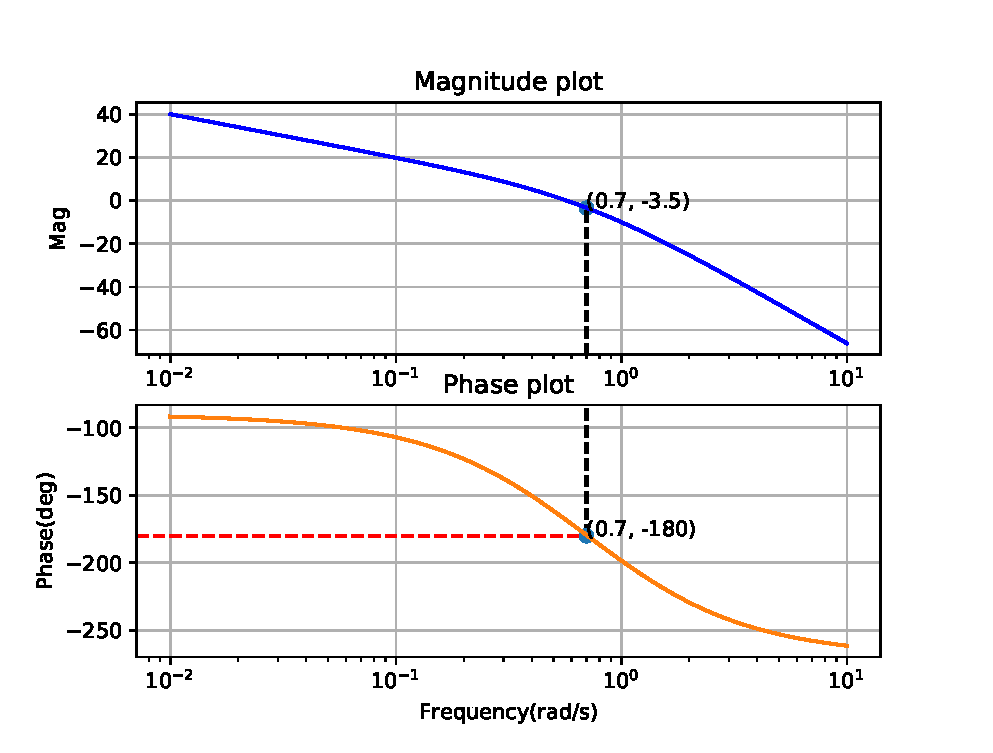
\includegraphics[width=\columnwidth]{./figs/ee18btech11016.eps}
  \caption{}
  \label{fig:ee18btech11016}
\end{figure}
%
Note that this nyquist plot is plotted when K=1.
\\
 
%\item  Use the Nyquist Stability criterion to determine the value of K since we know that the system in \eqref{eq:ee18btech11016_system} is stable.
%\\
%\solution  
\textbf{Nyquist criterion}-For the stable system :
\begin{align}
\label{eq:ee18btech11016_system_nyquist}
Z = P+N = 0,    
\end{align}
\begin{table}[!ht]
\centering
\input{./tables/ee18btech11016_table.tex}
\caption{}
\label{table:ee18btech11016}
\end{table}
\\
Since from the equation \eqref{eq:ee18btech11016_system_equation}, P = 2 as the number of poles on right hand side of s-plane is equal to 2 .So, for Z to be equal to 0 ,we have to choose the range of K such that N should be equal to -2.
\\
%\item Find the range of K from Nyquist criterion.
%\solution 
If we consider the Nyquist plot with K term i.e. of equation \eqref{eq:ee18btech11016_system_equation} , then it will cut x-axis at x = -0.254K , x = 0 and at x = 0.7873K (as we have nyquist graph at K=1, now we just need to multiply the intersected coordinates on x-axis by K). 
\\

So, we have to make sure that $(-1+\ j0)$ should be included in between x = -0.254K to x = 0, because then only N = -2 (as the no. of encirclements are 2 in anticlockwise direction in this case so N=-2)
\begin{align}
-0.254K < -1 < 0
\end{align}
So,
\begin{align}
K > \frac{1}{0.254}
\end{align}
i.e.
\begin{align}
K > 3.937
\end{align}
\\
Hence K $>$ 3.937 ensures that the system is stable as no. of poles on the right hand side of s-plane (in this case) is 0.
%\end{enumerate}
